\section{Specifications}
\label{firmware-specifications}

The firmware is basically an analog sampler, all it has to do is sample six analog
channels, add a header (to identify the beginning and check continuity) and send it
through USB. The following sections present the requirements of the system, details
about the selection of the microcontroller and how the signal acquisition parameters
(set by registers) were obtained.

\subsection{Requirements}
\begin{itemlist}
  \item Super cheap
  \item 6 analog channels (more precision is better)
  \item High sample rate (at least 10 kHz for each channel, but ideally 44 kHz or more)
  \item Fast USB support, to send the data with headers
\end{itemlist}
Based on this requirements the minimum transfer speed can be calculated. Considering
that a header will be set for every 252 samples (42 for each channel) and
it has 4 bytes (3 of identification - to assure it is the header and not some
data - and a counter). Previewing the worst case, each sample is 2 bytes long.
The transfer rate given by \autoref{usb-generic-rate-equation}.

\begin{equation}
  \label{usb-generic-rate-equation}
  transfer\ rate = \left( \frac{channels * \frac{bytes}{sample} * \frac{samples}{package} + header\ size}{\frac{samples}{package}}  \right ) * f_{s} [B/s]
\end{equation}

Considering that $f_{s}$ has to be somewhere between 10 kHz and 50 kHz, the transfer
rate numerical result is given by \autoref{usb-numerical-rate-equation}.

\begin{equation}
  \label{usb-numerical-rate-equation}
  transfer\ rate = \left( \frac{6 * 2 * 252 + 4}{252}  \right ) * f_{s} = 12.0159 * f_{s} = 120.159\ to\ 600.794 [kB/s]
\end{equation}

USB transfer speed is usually referred in Mbps, which gives a range between
0.97 and 4.8 Mbps. This is too high for serial communication (typical max of
1 Mbps for reliable transfers with no error) so we need to add a requirement for raw USB support, which allows \textit{bulk transfers}
that can a have transfer rate up to 12Mbps (USB full-speed standard).

It's still needed to choose or exact sample rate ($f_{s}$), but it is first necessary
select which hardware will be used.

\subsection{Microcontroller Selection}
There are too many microcontrollers that fit our requirements, but one of most popular
and cheap options available (by searching \"arm microcontroller board\" on AliExpress)
is the ARM from ST called STM32F103C8T6 \cite{STM32F103},
and that is why it was selected. 

It has eight 12 bits ADC inputs (with 2 parallel channels), DMA for the ADCs and USB full-speed support. It is
also relatively fast (72 MHz clock, 32 bits architecture). All this for under US\$ 2
in a developing board from China (the actual $\mu$C is under 0.2 U\$).
The board's pinout can be seen in \autoref{STM32F103-board}.

\begin{figure}[htb]
  \centering
  \caption{STM32F103C8T6 Board}
  \label{STM32F103-board}
  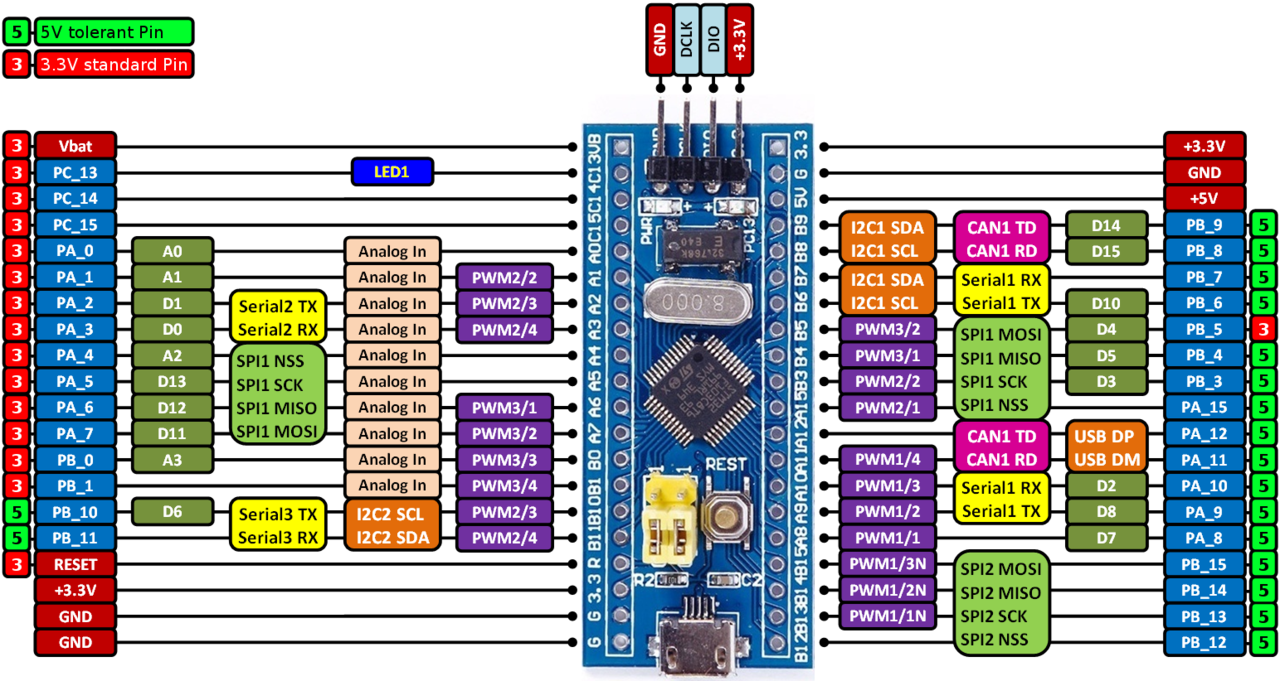
\includegraphics[scale=0.3]{images/STM32F103-board}
  \legend{Source: \citeonline{STM32F103-board-image}}
\end{figure}

\subsection{Sample Frequency}
\label{firmware-sample-frequency}
Usage of the ADCs for the selected $\mu$C can be optimized by using continuous sampling
mode in conjunction with DMA \cite[ch. 11]{STM32F103}. In this mode, the sample frequency is controlled by a register
that sets the \textit{convolution time}. The convolution time is the amount of time
the ADC takes to sample. The longer it is (more ADC clock cycles) the better the resulting precision.

The first variable chosen for this setup is the ADC clock, which is set by dividing
the $\mu$C clock by 2, 4, 6 or 8. The ADC also has a maximum clock of 14 MHz. Taking in
account the  $\mu$C clock of 72 MHz, the highest possible value for the ADC clock is 12 MHz,
which is set by a divider value of 6. 

The last value to be chosen is the mentioned convolution time ($T_{c}$ is calculated as the selected
value plus 12.5 ADC clock cycles), which gives a sample frequency calculate by \autoref{ADC-sampling-time}.

\begin{equation}
  \label{ADC-sampling-time}
  f_{s} = \frac{ADC\ clock}{T_{c} + 12.5}  * \frac{Parallel ADCs}{channels} = \frac{12}{T_{c} + 12.5}  * \frac{2}{6}\ [MHz]
\end{equation}

\autoref{ADC-sampling-frequencies} shows the calculated results for each possible
register value (using \autoref{ADC-sampling-time}). Based on it the chosen sampling
frequency is 47.619 kHz. By using \autoref{usb-numerical-rate-equation} we can also
calculate the actual data transfer rate (for all channels, including header),
resulting in a total of 572.185 kB/s. This last value will be used to test the USB communication.

\begin{table}[htb]
  \caption{ADC Sampling Frequencies}
  \label{ADC-sampling-frequencies}
  \begin{tabular}{c|c|c}
    \textbf{Register Value} & \textbf{Convolution Time [cycles]} & \textbf{Sampling Frequency [kHz]}\\
    \hline \hline
    000 & 1.5 & 285.71 \\
    \hline
    001 & 7.5 & 200 \\
    \hline
    010 & 13.5 & 153.85 \\
    \hline
    011 & 28.5 & 97.56 \\
    \hline
    100 & 41.5 & 74.07 \\
    \hline
    101 & 55.5 & 58.82 \\
    \hline
    \textbf{110} & \textbf{71.5} & \textbf{47.62} \\
    \hline
    111 & 239.5 & 15.87 \\
  \end{tabular}
  \legend{Source: authors}
\end{table}
